
\begin{figure}
\centering
  \mbox{
  	\subfloat[CPU time for IQS]{
		\label{fig:ctimeiqs}
		%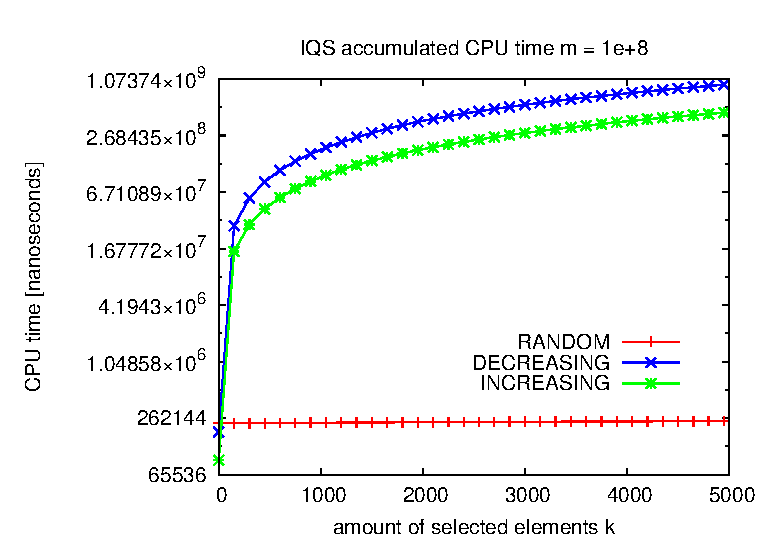
\includegraphics[height=6cm]{figures/ctimeiqs.eps}
		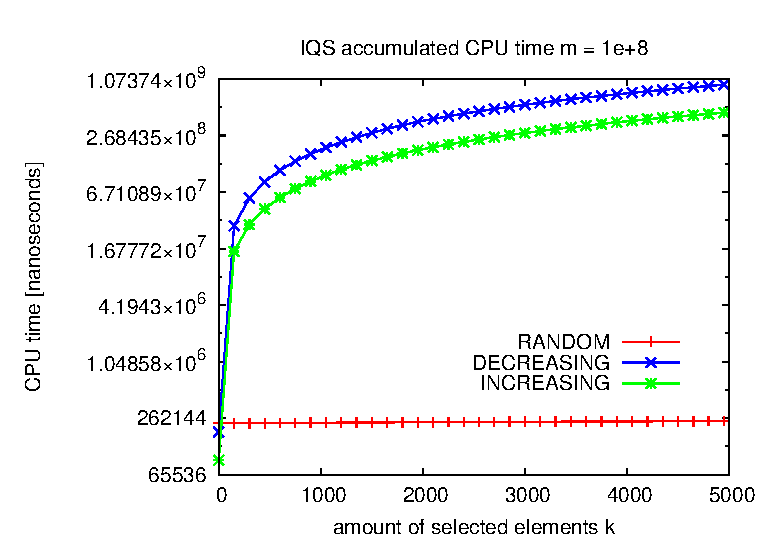
\includegraphics[width=.5\textwidth]{figures/ctimeiqs.eps}
	}
}
  \mbox{
  	\subfloat[CPU time for IIQS]{
		\label{fig:ctimeisiqs}
		%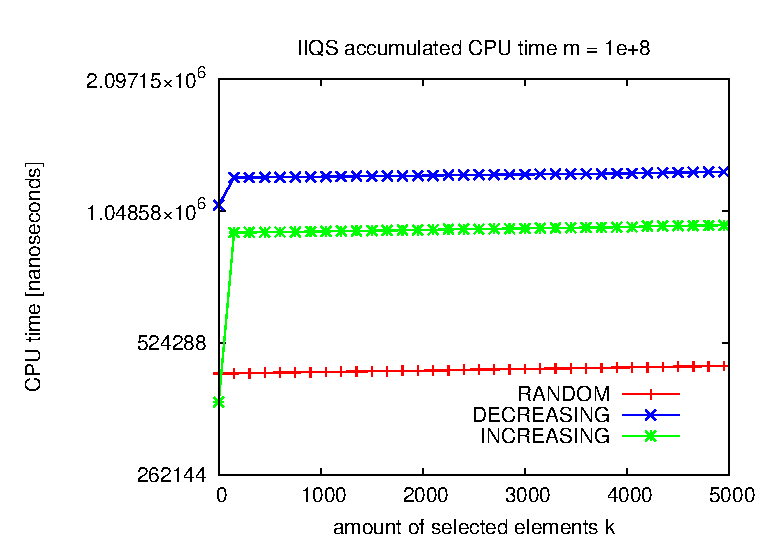
\includegraphics[height=6cm]{figures/ctimeiiqs.eps}
		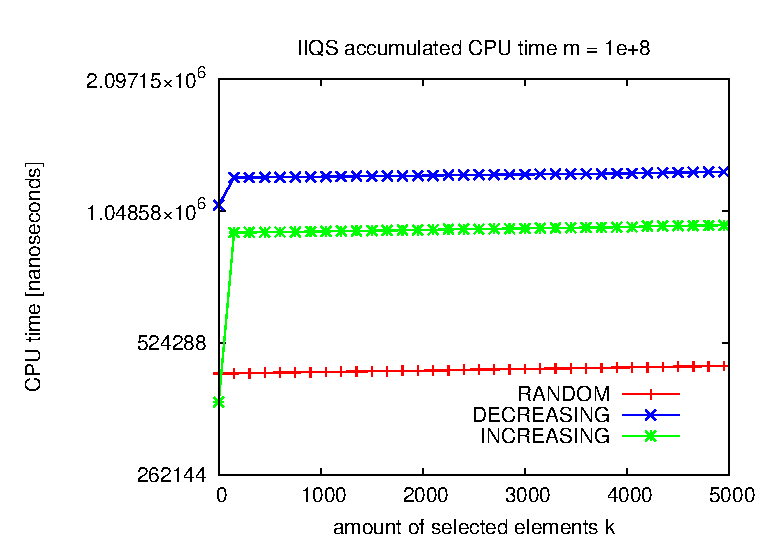
\includegraphics[width=.5\textwidth]{figures/ctimeiiqs.eps}
	}
}
  \mbox{
  	\subfloat[Stack size of IQS and IIQS]{
		\label{fig:stacksizesummary} 
		%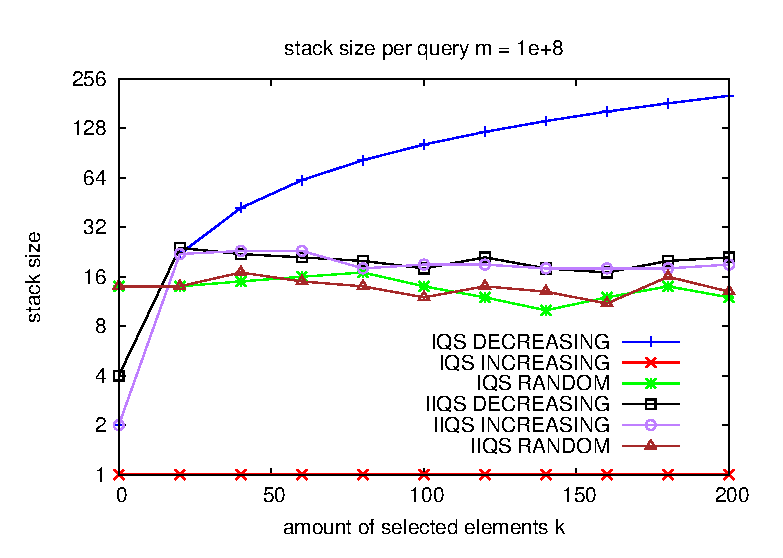
\includegraphics[height=6cm]{figures/ssizesummary.eps}
		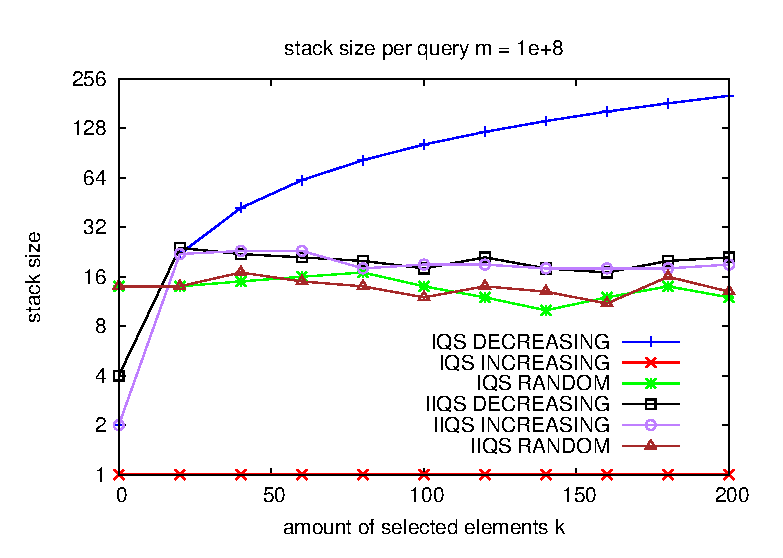
\includegraphics[width=.5\textwidth]{figures/ssizesummary.eps}
	}	
}

\caption{Performance comparison between IQS and IIQS as a function of the amount of searched elements $k$. Note the logscales in the plots.}\label{fig:performancecomparison}
\end{figure}